\subsubsection{04.02.2016}
\textit{\textbf{Time frame:}} 10:00-18:00 

The cover for bucket was tested and it was found out that the axis if rotation is placed too far from the bucket, so the trajectory of its movement is too wide. However, free space inside the robot was not as much as required, so it was decided to recreate the cover (figure \ref{Bucket2.5}, \ref{Bucket2.6}).

\begin{figure}[H]
	\begin{minipage}[h]{0.47\linewidth}
		\center{\includegraphics[scale=0.2]{3Engineering/5Team_meetings/days_of_meetings/2016.02.04/images/01}}
		\caption{Cover for bucket (opened)}
		\label{Bucket2.5}
	\end{minipage}
	\hfill
	\begin{minipage}[h]{0.47\linewidth}
		\center{\includegraphics[scale=0.2]{3Engineering/5Team_meetings/days_of_meetings/2016.02.04/images/02}}
		\caption{Cover for bucket (opened)}
		\label{Bucket2.6}
	\end{minipage}
\end{figure}

After the cover was improved, the bucket was installed onto the robot (figure \ref{Bucket2.7}).

\begin{figure}[H]
	\begin{minipage}[h]{1\linewidth}
		\center{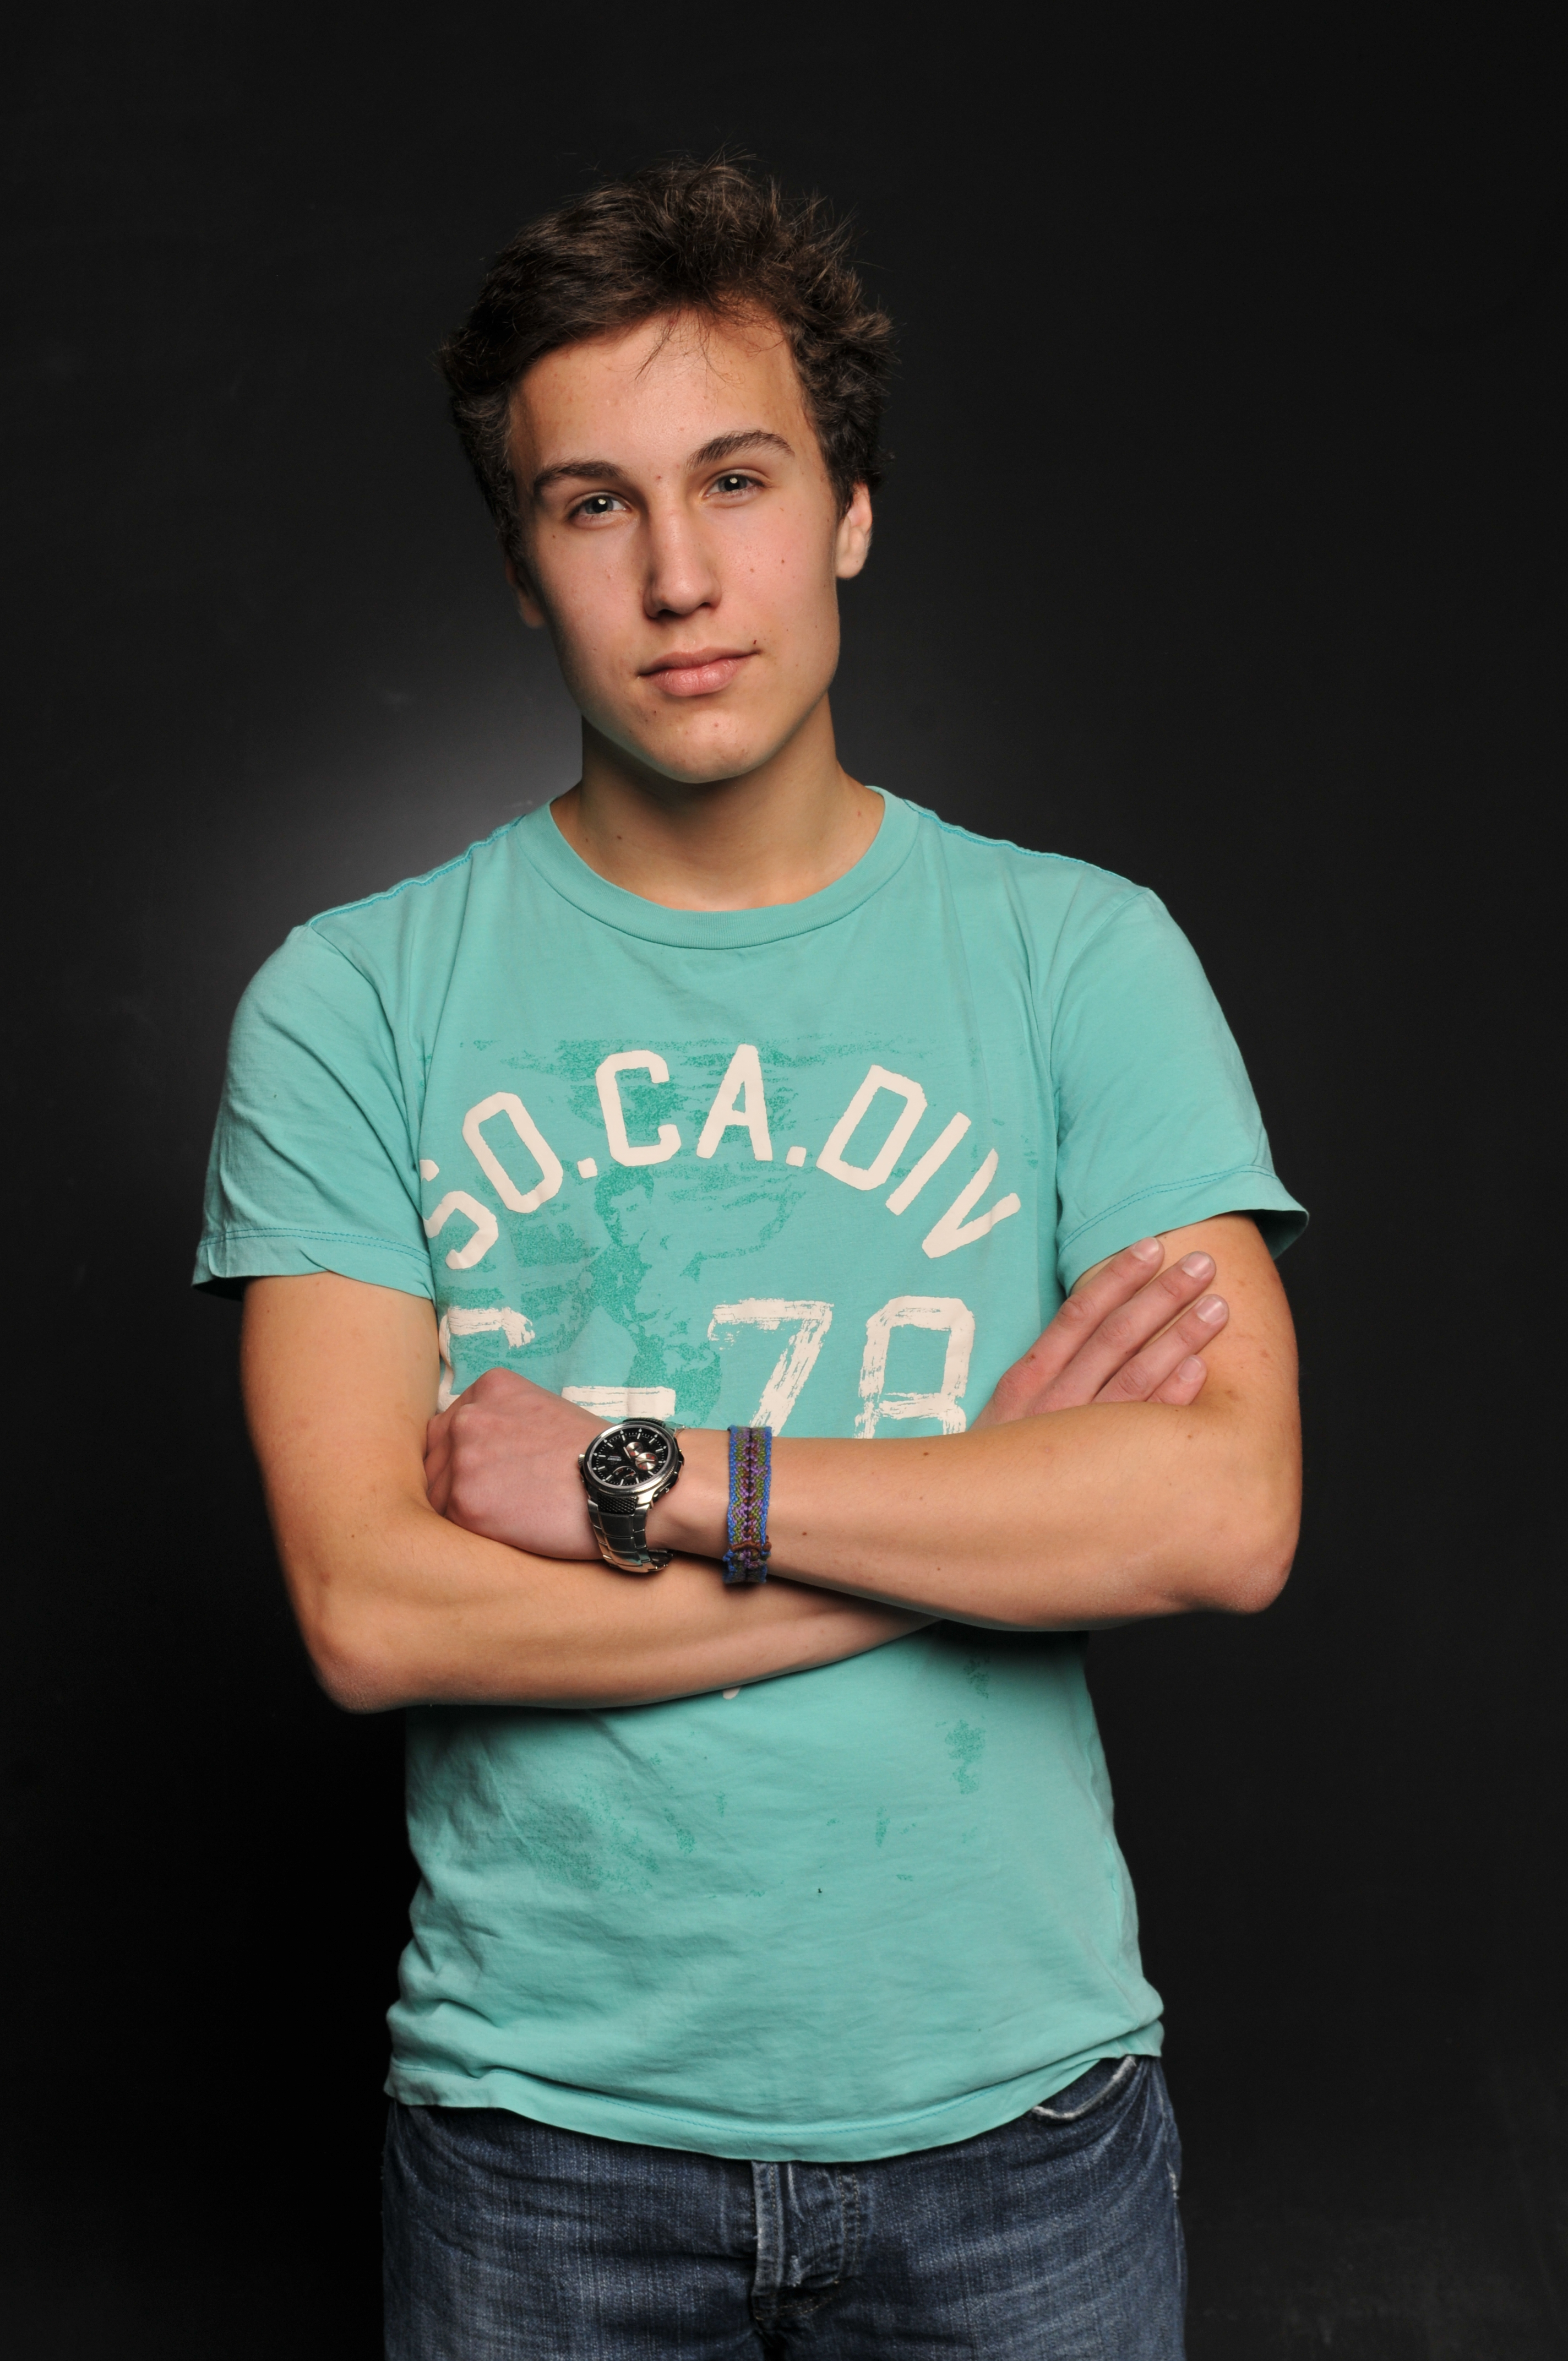
\includegraphics[scale=0.2]{3Engineering/5Team_meetings/days_of_meetings/2016.02.04/images/03}}
		\caption{Bucket fixed on the robot}
		\label{Bucket2.7}
	\end{minipage}
\end{figure}